%%
%% This is file `sample-manuscript.tex',
%% generated with the docstrip utility.
%%
%% The original source files were:
%%
%% samples.dtx  (with options: `all,proceedings,bibtex,manuscript')
%% 
%% IMPORTANT NOTICE:
%% 
%% For the copyright see the source file.
%% 
%% Any modified versions of this file must be renamed
%% with new filenames distinct from sample-manuscript.tex.
%% 
%% For distribution of the original source see the terms
%% for copying and modification in the file samples.dtx.
%% 
%% This generated file may be distributed as long as the
%% original source files, as listed above, are part of the
%% same distribution. (The sources need not necessarily be
%% in the same archive or directory.)
%%
%%
%% Commands for TeXCount
%TC:macro \cite [option:text,text]
%TC:macro \citep [option:text,text]
%TC:macro \citet [option:text,text]
%TC:envir table 0 1
%TC:envir table* 0 1
%TC:envir tabular [ignore] word
%TC:envir displaymath 0 word
%TC:envir math 0 word
%TC:envir comment 0 0
%%
%% The first command in your LaTeX source must be the \documentclass
%% command.
%%
% \documentclass[sigconf]{acmart}
\documentclass[manuscript,screen]{acmart}
%%
%% \BibTeX command to typeset BibTeX logo in the docs
\AtBeginDocument{%
  \providecommand\BibTeX{{%
    Bib\TeX}}}

%% Rights management information.  This information is sent to you
%% when you complete the rights form.  These commands have SAMPLE
%% values in them; it is your responsibility as an author to replace
%% the commands and values with those provided to you when you
%% complete the rights form.
\setcopyright{acmlicensed}
\copyrightyear{2025}
\acmYear{2025}
% \acmDOI{XXXXXXX.XXXXXXX} %% No DOI provided
%% These commands are for a PROCEEDINGS abstract or paper.
% \acmConference[Conference acronym 'XX]{Make sure to enter the correct
%   conference title from your rights confirmation email}{June 03--05,
%   2025}{Woodstock, NY}
%%
% \acmISBN{978-1-4503-XXXX-X/2025/06} %% No ISBN provided

%%
%% For managing citations, it is recommended to use bibliography
%% files in BibTeX format.
%%
%% You can then either use BibTeX with the ACM-Reference-Format style,
%% or BibLaTeX with the acmnumeric or acmauthoryear sytles, that include
%% support for advanced citation of software artefact from the
%% biblatex-software package, also separately available on CTAN.
%%
%% Look at the sample-*-biblatex.tex files for templates showcasing
%% the biblatex styles.
%%

%%
%% The majority of ACM publications use numbered citations and
%% references.  The command \citestyle{authoryear} switches to the
%% "author year" style.
%%
%% If you are preparing content for an event
%% sponsored by ACM SIGGRAPH, you must use the "author year" style of
%% citations and references.
%% Uncommenting
%% the next command will enable that style.
%%\citestyle{acmauthoryear}

%%
%% end of the preamble, start of the body of the document source.
\begin{document}

%%
%% The "title" command has an optional parameter,
%% allowing the author to define a "short title" to be used in page headers.
\title{A Spatially-Aware Search Engine for Textual Content in Images}

%%
%% The "author" command and its associated commands are used to define
%% the authors and their affiliations.
\author{Pranav Ramesh}
\email{pranavramesh@college.harvard.edu}
% \orcid{XXXX-XXXX-XXXX-XXXX} %% Add ORCID if available
\affiliation{%
  \institution{Harvard University}
  \city{Cambridge}
  \state{MA}
  \country{USA}
}

\author{Mohamed Zidan Cassim}
\email{mzcassim@college.harvard.edu}
% \orcid{XXXX-XXXX-XXXX-XXXX} %% Add ORCID if available
\affiliation{%
  \institution{Harvard University}
  \city{Cambridge}
  \state{MA}
  \country{USA}
}

\author{Giovanni D'Antonio}
\email{giovannidantonio@college.harvard.edu}
% \orcid{XXXX-XXXX-XXXX-XXXX} %% Add ORCID if available
\affiliation{%
  \institution{Harvard University}
  \city{Cambridge}
  \state{MA}
  \country{USA}
}

%%
%% By default, the full list of authors will be used in the page
%% headers. Often, this list is too long, and will overlap
%% other information printed in the page headers. This command allows
%% the author to define a more concise list
%% of authors' names for this purpose.
\renewcommand{\shortauthors}{Ramesh et al.}

%%
%% The abstract is a short summary of the work to be presented in the
%% article.
\begin{abstract}
  Standard image search engines often treat text within images as secondary metadata or ignore its spatial location. This limits users' ability to find images based on text appearing in specific visual areas. We present a spatially-aware textual image search engine designed to address this limitation. Our approach utilizes an inverted index mapping text n-grams to their normalized bounding box coordinates within images. Queries consist of text and an optional spatial region. Relevance scoring combines spatial factors (Intersection over Union - IoU and proximity) with n-gram length, weighted according to configurable parameters. To facilitate development and evaluation, we developed a pipeline for generating synthetic datasets with controlled text placement and ground truth. We evaluated our system against non-spatial baselines (keyword-only and n-gram-only) using Mean Average Precision (MAP) and Precision@k (P@k) on this synthetic data. Results demonstrate statistically significant improvements in ranking quality for both n-gram usage over keywords (MAP 0.21 vs 0.03) and spatial awareness over n-grams alone (MAP 0.67 vs 0.21), validating the effectiveness of incorporating both n-grams and spatial context. A visualization tool was also developed to aid in understanding search results.
\end{abstract}

%%
%% The code below is generated by the tool at http://dl.acm.org/ccs.cfm.
%% Please copy and paste the code instead of the example below.
%%
% \begin{CCSXML}
% <ccs2012>
%  <concept>
%   <concept_id>10010520.10010553.10010562</concept_id>
%   <concept_desc>Computer systems organization~Embedded systems</concept_desc>
%   <concept_significance>500</concept_significance>
%  </concept>
%  <concept>
%   <concept_id>10010520.10010575.10010755</concept_id>
%   <concept_desc>Computer systems organization~Redundancy</concept_desc>
%   <concept_significance>300</concept_significance>
%  </concept>
%  <concept>
%   <concept_id>10010520.10010553.10010554</concept_id>
%   <concept_desc>Computer systems organization~Robotics</concept_desc>
%   <concept_significance>100</concept_significance>
%  </concept>
%  <concept>
%   <concept_id>10003033.10003083.10003095</concept_id>
%   <concept_desc>Networks~Network reliability</concept_desc>
%   <concept_significance>100</concept_significance>
%  </concept>
% </ccs2012>
% \end{CCSXML}

\ccsdesc[500]{Information systems~Information retrieval}
\ccsdesc[500]{Information systems~Retrieval tasks and goals~Image search}
\ccsdesc[300]{Computing methodologies~Computer vision~Object detection}
\ccsdesc[300]{Information systems~Indexing}
\ccsdesc[100]{Computing methodologies~Document analysis and representation~Optical character recognition}
\ccsdesc[100]{Computing methodologies~Image processing}
\ccsdesc[100]{Information systems~Search engine architectures and scalability}

%%
%% Keywords. The author(s) should pick words that accurately describe
%% the work being presented. Separate the keywords with commas.
\keywords{image search, text localization, spatial search, n-grams, OCR, information retrieval}

\received{20 April 2025}
\received[revised]{12 May 2025}
\received[accepted]{5 June 2025}

%%
%% This command processes the author and affiliation and title
%% information and builds the first part of the formatted document.
\maketitle

\section{Introduction}

\subsection{Problem Statement}

Images frequently contain rich textual information, such as signs, labels, headlines, logos, or embedded text in documents and screenshots. Traditional image search systems primarily focus on visual features or global textual tags, often failing to leverage the specific content and location of text within the image. Users cannot easily query for images containing specific text within a particular visual region (e.g., "find photos with 'SALE' in the top-right corner" or "show screenshots where 'error message' appears near the bottom"). This lack of spatial awareness limits the precision and utility of text-based image retrieval.

\subsection{Motivation}

The ability to search for text within specific spatial regions of images unlocks numerous applications across multiple domains. Document analysis benefits by enabling users to find specific sections or figures in scanned documents based on headings or captions in known layout areas. In retail and e-commerce, such technology facilitates locating product images where price or discount tags appear in particular locations relative to the product. Scene understanding applications can identify street signs, shop names, or specific labels within photographs of complex scenes with greater accuracy when spatial relationships are considered. UI/UX researchers can leverage spatial text search to analyze screenshots and find instances where specific labels or error messages appear in certain interface elements. Additionally, accessibility is enhanced by enabling visually impaired users to query not just what text appears in an image, but where it is located.

To illustrate the practical utility more concretely, consider a case study in \textbf{Automated Data Entry from Scanned Documents}. Imagine processing a high volume of scanned invoices or receipts for accounting. While Optical Character Recognition (OCR) can extract all text from an image, accurately identifying the \textit{semantic role} of specific text snippets (e.g., distinguishing the "Total Amount" from line item prices, or the "Invoice Date" from a "Payment Due Date") is a significant challenge due to the wide variety of document layouts. A traditional keyword search for terms like "Total" or for date patterns might yield multiple ambiguous candidates scattered across the document.

This is where spatially-aware search offers a distinct advantage. By leveraging common layout conventions, the system can target queries to specific regions. For example, a query searching for text matching a monetary amount pattern (e.g., \verb|\$\d+\.\d{2}|) \textit{specifically within the normalized coordinates corresponding to the bottom-right quadrant} of the document is highly likely to isolate the final \textbf{Total Amount}. Similarly, querying for date-like text primarily within the \textit{top-right quadrant} can reliably extract the \textbf{Invoice Date}. This targeted spatial querying drastically reduces ambiguity compared to context-agnostic text search, significantly simplifying the development of robust automated data entry pipelines without requiring complex template matching or sophisticated layout analysis models for every document variant. It demonstrates how spatial awareness can act as a powerful heuristic for semantic disambiguation in structured documents.

Existing methods often rely on whole-image tags or complex scene understanding models that may not precisely capture localized text queries. A dedicated system focusing on spatial text search promises higher precision and user control for these tasks.

\subsection{Proposed Solution \& Contributions}

To address the limitations of traditional methods, we propose and implement \textbf{SATIAS (Spatially-Aware Textual Image Search)}, a search engine designed to retrieve images based not only on \textit{what} text they contain but also \textit{where} that text is located. The core idea is to move beyond simple keyword matching by creating an index that explicitly links textual content (represented as n-grams, typically sequences of 1 to 3 words) to its precise spatial location within each image. This is achieved by building an inverted index where keys are text n-grams and values are lists of occurrences, each storing the \verb|image_id| and the n-gram's \textbf{normalized bounding box} coordinates (percentages of image width/height) to ensure scale and aspect-ratio invariance. User queries can specify both a \verb|query_text|, which is parsed into n-grams, and an optional target \textbf{spatial region}, also represented as a normalized bounding box. Candidate images containing matching n-grams are retrieved via the index, and each potential match is evaluated using a novel, configurable scoring mechanism. This scoring combines \textbf{spatial relevance}—calculated as a weighted sum of \textbf{Intersection over Union (IoU)} for overlap and \textbf{centroid proximity} for nearness between the query region and the n-gram box—with \textbf{textual relevance}, where matches involving longer n-grams contribute more significantly. The relative importance of IoU versus proximity can be tuned via configuration weights. Finally, scores are aggregated per image, and the results are ranked to provide the user with images where the desired text appears in the specified location.

This paper details the design, implementation, and rigorous evaluation of the SATIAS system. Our primary contributions include: (1) the \textbf{novel algorithm design} itself, particularly the use of normalized coordinates for indexing and the hybrid spatial scoring function combining weighted IoU and proximity; (2) a robust and parallelized \textbf{synthetic data generation pipeline} (\verb|data_generation/|) that creates large datasets with precise ground-truth bounding boxes and targeted queries, crucial for controlled offline evaluation independent of OCR errors; (3) a modular Python \textbf{system implementation} (\verb|search_engine/|) encompassing indexing, flexible query parsing, spatial calculations, and search logic; (4) a \textbf{rigorous quantitative evaluation} framework (\verb|evaluate.py|) using MAP@k and P@k metrics to compare SATIAS against keyword-only and n-gram-only baselines on the synthetic data, including statistical significance testing (Wilcoxon signed-rank test); and (5) an \textbf{interactive visualization tool} (\verb|visualize_search.py|) with a GUI that allows users to execute searches and inspect results with overlays showing query regions and color-coded n-gram bounding boxes based on IoU, aiding qualitative analysis and debugging.

\begin{figure}[ht]
    \centering
    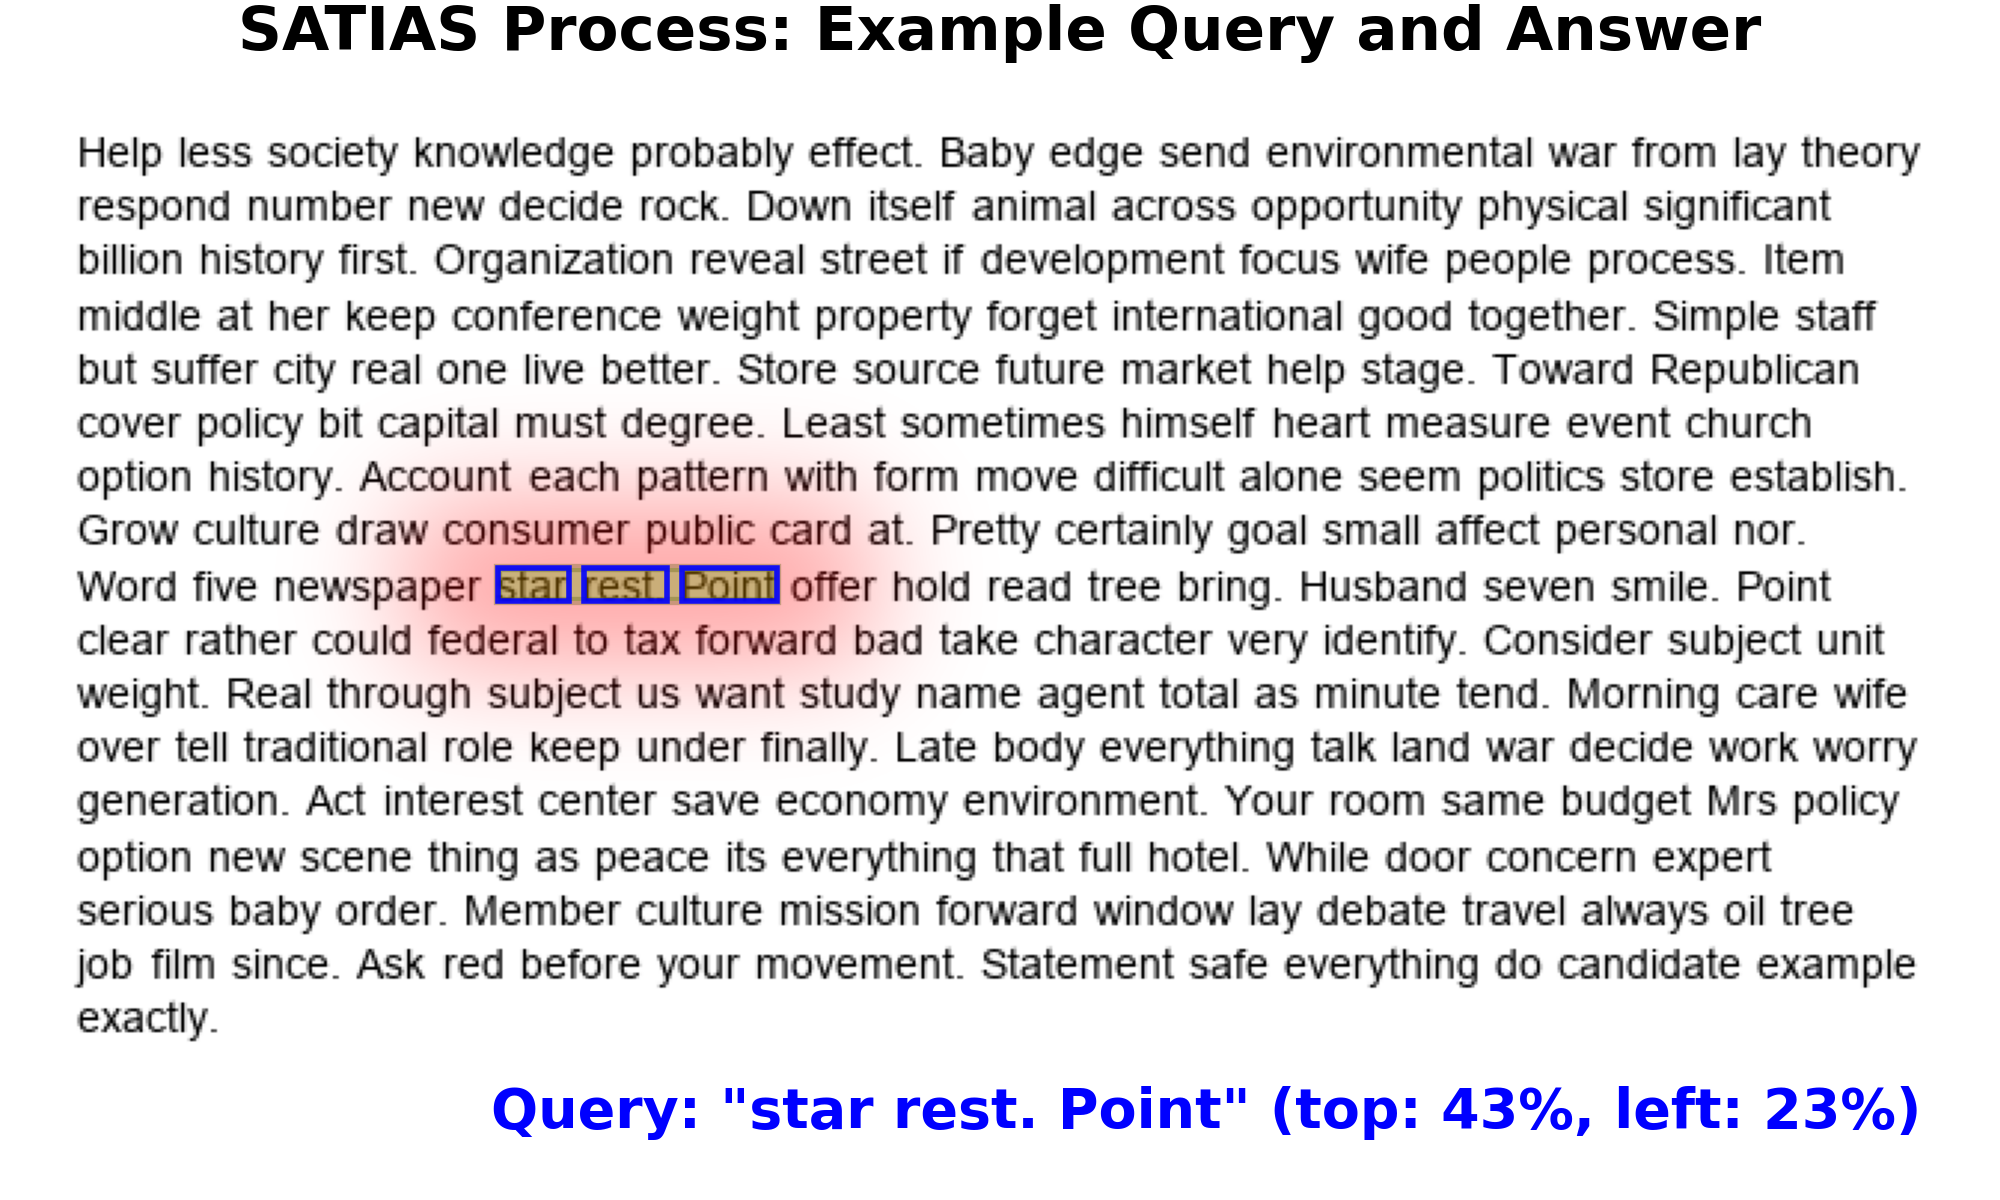
\includegraphics[width=0.95\linewidth]{satias_example.png}
    \caption{Illustration of the SATIAS process. The blue boxes indicate the n-gram query region, the heat overlay shows the answer area, and the query text at bottom right demonstrates a location-aware search.}
    \label{fig:satias-process}
\end{figure}

\section{Prior Work}

The challenge of searching for textual content within images, potentially constrained by location, has been explored from various perspectives. Our work draws upon foundational concepts while offering a specific, geometrically focused solution.

\subsection{Foundational and Explicit Spatial Methods}

\textbf{Foundational Text-in-Image Search:} Early research, such as that by Manmatha et al. (UMass CIIR, 2000) \cite{Manmatha00}, focused on the fundamental problems of detecting, extracting (via OCR), and indexing text found within images for keyword-based retrieval. These systems laid the groundwork but typically treated text as document-level metadata or lacked mechanisms for precise spatial querying. Our system builds on this by explicitly indexing the \textit{location} of extracted text (n-grams) and enabling queries against these locations.

\textbf{Spatial-Semantic Approaches:} More recent work has integrated spatial reasoning with semantic understanding. Mai et al. (CVPR 2017) \cite{Mai17} proposed a spatial-semantic image search framework where users define semantic layouts on a canvas, and a CNN synthesizes corresponding visual features for retrieval. This differs from our approach, which focuses narrowly on matching the precise geometric location (bounding box) of specific text n-grams provided in the query, rather than interpreting broader semantic layouts.

\subsection{The Rise of MLLMs in Spatial Grounding}

Recent years have seen a significant shift towards utilizing Multimodal Large Language Models (MLLMs) for tasks involving spatial grounding. These models, such as KOSMOS-2 \cite{Huang24} and Groma \cite{Yin24}, aim to integrate visual perception, language comprehension, and spatial reasoning within unified architectures, often trained on web-scale datasets \cite{Huang24}.

\textbf{Approach:} Instead of explicit geometric indexing and scoring like our system, MLLMs typically handle spatial information implicitly through learned mechanisms. These mechanisms include using location tokens where continuous bounding box coordinates are discretized into special tokens integrated into the language model's vocabulary \cite{Huang24}, leveraging cross-modal attention mechanisms to learn correlations between text and image regions, and utilizing joint embedding spaces that align visual regions and textual descriptions, implicitly encoding spatial relationships.

\textbf{Comparison to Our System:} Compared to our system, MLLMs offer distinct advantages and disadvantages. MLLMs possess strong semantic understanding derived from their underlying LLMs, enabling them to handle synonyms, paraphrasing, and complex natural language queries describing spatial relations (e.g., "the book to the left of the lamp") \cite{Huang24, Yin24}, a capability our exact n-gram matching system lacks. However, the reasoning process of MLLMs is often opaque ("black box"), whereas our system, using explicit IoU and proximity calculations, offers greater interpretability and direct control via tunable weights. Additionally, training state-of-the-art MLLMs for grounding requires massive datasets (like the GRIT dataset used for KOSMOS-2 \cite{Huang24}) and significant computational resources for pre-training and fine-tuning \cite{Yin24}. Our indexing approach, while requiring OCR, may have different data dependencies, primarily needing the images themselves rather than extensive grounded text-region pairs for initial training. This trend towards MLLMs highlights a different paradigm for spatial understanding, trading explicit geometric control for learned semantic richness and query flexibility, albeit with associated challenges in interpretability and data requirements.

\subsection{Enabling Technologies}

\textbf{Text Spotting:} Accurate detection and bounding box generation are critical prerequisites for any text-in-image search system. The field has advanced to handle arbitrary text shapes using segmentation, contour embedding, Bezier curves (ABCNet), Mask R-CNN, or sequential deformation. However, bounding box inaccuracy remains a challenge for real-world geometric scoring.

\textbf{Indexing:} Scalability requires efficient indexing structures. While our approach uses an in-memory inverted index, spatial databases traditionally use R-Trees/Quadtrees, often combined with inverted indexes in hybrid structures. Recent Learned Sparse Retrieval (LSR) methods (e.g., STAIR \cite{Chen23}, Cao et al. \cite{Cao23}, Bai et al. \cite{Bai24}) map dense embeddings to sparse lexical vectors compatible with inverted indexes, offering a promising direction for scalable multimodal retrieval.

\subsection{Contributions}

Our work occupies a niche focused on precise, spatially constrained retrieval of specific text n-grams. Compared to the prior work, our contributions are:

\begin{enumerate}
\item The use of an efficient inverted index mapping n-grams directly to normalized bounding boxes
\item A tunable spatial scoring function explicitly combining geometric overlap (IoU) and centroid proximity, offering direct control over spatial relevance criteria
\item A dedicated synthetic data generation pipeline and evaluation methodology designed to rigorously assess the performance of spatial text localization, isolating it from OCR errors and providing targeted spatial query scenarios
\end{enumerate}

Our approach provides a simple, interpretable method for precise geometric localization of exact text n-grams within rectangular regions. Its strengths are direct geometric control and the synthetic data pipeline for evaluation. Key limitations include dependence on OCR accuracy, lack of semantic understanding (unlike VSE/attention models), limited query expressiveness (compared to canvas/trace/relational queries), and scalability issues addressed by spatial/hybrid/LSR indexing. It represents a valuable baseline but stands apart from dominant deep learning trends emphasizing semantics and learned alignments.

\subsection{Comparison of Approaches}

Table~\ref{tab:approaches} provides a comprehensive comparison of various spatially-aware image-text retrieval approaches, highlighting the distinctive positioning of our system among existing methods.

\begin{table*}
  \caption{Comparison of Spatially-Aware Image-Text Retrieval Approaches}
  \label{tab:approaches}
  \begin{tabular}{p{2.8cm}p{2.8cm}p{4.5cm}p{3.4cm}}
    \toprule
    Approach & Query Type & Key Characteristics & Strengths/Weaknesses \\
    \midrule
    Foundational Text-in-Image (Manmatha et al., 2000) & Keywords & Text as document metadata; Inverted Index; Keyword matching & (+) Established base approach \\
    & & & (-) No spatial awareness \\
    \midrule
    Explicit Spatial-Semantic (Mai et al., 2017) & Text-boxes on canvas & User-defined layout; Visual Feature Index; Feature similarity & (+) Flexible canvas input \\
    & & & (-) Less precise text matching \\
    \midrule
    VSE / Attention Models & Text Query & Implicit spatial via embeddings; Learned attention mechanisms & (+) Strong semantic understanding \\
    & & & (-) No explicit spatial queries \\
    \midrule
    MLLMs (KOSMOS-2, Groma) & Natural Language & Learned mechanisms; End-to-end approach & (+) Semantic flexibility \\
    & & & (-) Black-box reasoning \\
    \midrule
    Our Approach & N-grams + Optional Region & Normalized Bounding Boxes; Explicit IoU + proximity scoring & (+) Interpretable; Precise \\
    & & & (-) Limited semantics; OCR dependent \\
  \bottomrule
\end{tabular}
\end{table*}

\section{Methodology}

Our system comprises two main phases: offline indexing and online query processing/search.

\subsection{Core Algorithm Overview}

The system first preprocesses a collection of images (or uses pre-computed metadata in our synthetic case) to build an inverted index. This index maps text n-grams to a list of all locations (image ID and normalized bounding box) where they appear. During online search, a user query (text + optional region) is processed. N-grams are extracted from the query text. The inverted index is used to retrieve candidate image locations matching these n-grams. Each match is scored based on n-gram length and spatial relevance relative to the query region. Scores are aggregated per image, and results are ranked.

\subsection{Indexing Phase}

\paragraph{Objective} Create an efficient lookup structure for n-gram occurrences and their spatial locations.

\paragraph{Process} The indexing phase creates a mapping between textual content and its spatial location across all images in the collection. It begins with the processing of image metadata, which can be derived from OCR output or, in our case, from pre-calculated metadata containing words, n-grams, and their precise pixel bounding boxes. For each n-gram in each image, the system normalizes its pixel bounding box coordinates from absolute pixel values \verb|[t, l, b, r]| to percentage-based coordinates \verb|[norm_t, norm_l, norm_b, norm_r]| relative to the image dimensions. This normalization step is crucial as it ensures that spatial comparisons remain consistent across images of varying resolutions and aspect ratios, enabling reliable spatial querying across diverse image sources.

The core data structure employed is an inverted index mapping n-grams to their occurrences. Each key in this index is a text n-gram string, and the corresponding value is a list of occurrences, where each occurrence contains an image identifier and normalized bounding box coordinates. As the system processes each n-gram from the input data, it appends a new entry containing the image identifier and normalized bounding box to the list associated with that n-gram text. Once constructed, the entire index is serialized and saved to persistent storage, allowing efficient loading in subsequent search sessions without rebuilding the index.

\subsection{Query Processing}

\paragraph{Objective} Convert user input into a format suitable for searching the index.

\paragraph{Process} The query processing stage transforms raw user input into structured data that can be efficiently matched against the inverted index. This process handles two key components: the query text and an optional spatial region specification. For the textual component, the system divides the input query text into individual words and generates all possible n-grams within the configured range (from the minimum to maximum n-gram length). This n-gram extraction mirrors the approach used during indexing, ensuring consistency between indexed content and query terms.

For the spatial component, the system parses an optional region string parameter, which can specify a target area within images using various formats (e.g., \verb|"top: 10-30, left: 50-70"|). This parsing interprets different notation styles for specifying top, left, bottom, and right boundaries or ranges as percentages of image dimensions. The parser performs validation on these values and handles edge cases gracefully. If the spatial region string is missing, invalid, or cannot be parsed, the system defaults to using the full image area represented as normalized coordinates \verb|[0.0, 0.0, 100.0, 100.0]|, effectively conducting a whole-image search. After processing both components, the function returns the complete query representation: a list of extracted query n-grams and a single normalized query bounding box ready for the search phase.

\subsection{Search and Ranking}

\paragraph{Objective} Retrieve and rank images based on textual and spatial relevance.

\paragraph{Process} The search process begins with the initialization of an image score accumulator that will track the relevance score for each candidate image. For each query n-gram, the system performs a lookup in the inverted index to retrieve all matching occurrences across the indexed images. When a query n-gram is found, the algorithm iterates through each occurrence, represented as a tuple of image identifier and normalized bounding box, and calculates its contribution to the overall image score.

The scoring mechanism first determines the appropriate spatial relevance component. For baseline non-spatial searches or when the query doesn't specify a region of interest (using the default full-image bounding box), this component is set to 1.0, effectively ignoring spatial factors. However, when processing spatially-aware queries with specific target regions, the system employs a sophisticated dual-metric approach. It calculates the Intersection over Union (IoU) between the query region and the n-gram bounding box, which quantifies the degree of overlap. Simultaneously, it computes a proximity score based on the distance between centroids of the query and n-gram regions, using an exponential decay function that rewards closer matches. These two metrics are then combined into a single spatial score using configurable weights (typically equal weights of 0.5 each). This hybrid approach effectively addresses the limitations of using either metric in isolation—IoU fails to reward nearby non-overlapping matches, while proximity alone would ignore the extent of overlap and relative sizes.

The algorithm then weights this spatial relevance by the n-gram length, recognizing that longer matching phrases should contribute more significantly to relevance than shorter ones. This weighted score is added to the accumulated score for the corresponding image. After processing all query n-grams and their occurrences, the system sorts the image scores in descending order and returns a ranked list of images with their relevance scores, representing the most relevant images for the given query.

This scoring approach provides a balance between textual and spatial relevance, with the configurable weights offering flexibility to adjust the importance of exact overlap versus general proximity based on specific application needs. The n-gram length weighting further enhances discrimination, favoring images containing more specific, longer matching phrases over those with only short, potentially more ambiguous matches.

\subsection{Synthetic Dataset Generation}

\paragraph{Motivation} Generating a synthetic dataset provided several key advantages for our research. The approach allowed us precise control over text content, layout, and repetition within the images. We were able to obtain perfect pixel-level bounding boxes for every word and n-gram, effectively eliminating OCR errors as a confounding variable during algorithm development. This dataset generation also facilitated automatically creating queries with known ground truth target images and specific spatial relationships (overlap, proximity, etc.) to systematically test different scoring scenarios. Additionally, the synthetic approach offered scalability by efficiently generating large datasets (thousands of images, tens of thousands of queries) using parallel processing.

\paragraph{Process} The synthetic dataset generation process began with centralized configuration controlling parameters like image dimensions, number of images, font settings, text density, repetition control, word distinctiveness, n-gram range, and query generation. The core logic first created a pool of unique sentences to ensure controlled repetition of words and phrases across different images. For each image, we created a blank canvas and selected a random subset of sentences from the pool. We probabilistically injected specific test phrases (e.g., "special offer") multiple times at random locations within the selected text, and replaced some common words with more distinctive words to aid later visual inspection and analysis. Words were then drawn onto the image sequentially (top-down, left-right), handling line wrapping based on margins and word width, with text allowed to bleed off the bottom edge to ensure full vertical coverage. Crucially, we calculated the precise pixel bounding box \verb|[top, left, bottom, right]| for each individual word before drawing and stored this information.

After generating the words and their positions, we calculated all n-grams within the configured range (e.g., 1 to 3 words) for each image. For each n-gram, we determined the union bounding box (in pixels) based on the exact pixel bounding boxes of its constituent words. The query generation process then created a set number of queries for each image by selecting a random n-gram already placed in that image as the textual target, with its location serving as the ground truth. We randomly chose a query region type based on the configured distribution (e.g., No Region, Exact Match, High IoU, Low IoU, Nearby, Distant) and generated a corresponding normalized query region based on the target n-gram's location and the chosen type. To maximize efficiency, we parallelized the generation process across multiple CPU cores.

\paragraph{Output} The generation pipeline produced several essential outputs: the synthetic images themselves, comprehensive metadata containing details about each image and lists of all words and n-grams within it along with their exact pixel bounding boxes, and a queries dataset containing all generated queries. Each query record includes a query identifier, ground truth image identifier, query text, normalized target region coordinates, ground truth bounding boxes for the text, and information about how the query region was created relative to the target text. This structured output provided all necessary information for training and evaluating our spatial search algorithms.

\section{Evaluation}

We conducted a quantitative evaluation to assess the performance of the spatially-aware search engine compared to relevant non-spatial baselines, using the generated synthetic dataset.

\subsection{Evaluation Setup}

The evaluation utilized a large synthetic dataset consisting of 50,000 queries derived from 2,000 generated images. For each query, we defined the single "relevant" image as the one specified in the query record—specifically, the image from which the query's target n-gram was originally sampled. All other images were considered non-relevant for that query. We compared three distinct configurations in our evaluation: (1) the full Spatial N-gram algorithm, which combines spatial scoring (IoU + proximity with balanced weights, typically 0.5/0.5) and n-gram length weighting; (2) an N-gram Baseline that ignores the query region and effectively ranks based only on text match (n-gram presence) and n-gram length to isolate the effect of n-grams compared to simple keywords; and (3) a Keyword Baseline representing a rudimentary non-spatial search that breaks the query text into unique words and scores images based simply on the count of matching words found anywhere in the image, ignoring both n-grams and location to serve as a fundamental baseline. All metrics were calculated using a cutoff of k=10.

\subsection{Evaluation Metrics}

Our evaluation employed several standard information retrieval metrics to comprehensively assess the effectiveness of the retrieval approaches. Mean Reciprocal Rank (MRR) measured the average of the reciprocal ranks of the first relevant result across all queries, providing insight into how quickly a user would find the first relevant result. Mean Average Precision (MAP) calculated the mean of the average precision scores for each query, offering a single-figure measure of quality across recall levels. Precision at k (P@k) measured the proportion of relevant documents in the top k results, directly reflecting precision from a user's perspective when viewing a limited number of results. We also calculated recall at various cutoffs to measure the fraction of relevant documents retrieved, and normalized Discounted Cumulative Gain (nDCG) to evaluate the usefulness of the ranking based on the graded relevance of results. Additionally, we computed Success@k, representing the percentage of queries where at least one relevant document appeared in the top k results. For this application, Success@1 was particularly significant as it indicated the proportion of queries where the algorithm successfully retrieved the exact desired image as the top result.

\subsection{Results}

The evaluation was conducted on a dataset containing 50,000 queries with a cutoff of k=10. Table~\ref{tab:results} summarizes the performance metrics for all three approaches.

\begin{table*}[t]
  \caption{Performance Comparison of Search Methods}
  \label{tab:results}
  \begin{tabular}{lccc}
    \toprule
    \textbf{Metric} & \textbf{Spatial N-gram} & \textbf{N-gram Baseline} & \textbf{Keyword Baseline} \\
    \midrule
    MAP@10 (Max: 1.0) & 0.6711 & 0.2110 & 0.0294 \\
    P@10 (Max: 0.1) & 0.0795 & 0.0324 & 0.0054 \\
    \bottomrule
  \end{tabular}
\end{table*}

\paragraph{Statistical Analysis}

To assess the significance of these results, we performed pairwise Wilcoxon signed-rank tests on the Average Precision (AP) scores for each query. The following p-values were obtained:

\begin{itemize}
    \item \textbf{Spatial N-gram vs. N-gram Baseline:} p-value = 0.0000
    \item \textbf{N-gram Baseline vs. Keyword Baseline:} p-value = 0.0000
    \item \textbf{Spatial N-gram vs. Keyword Baseline:} p-value = 0.0000
\end{itemize}

All p-values are less than 0.0001, indicating that the observed differences are highly statistically significant. The 95\% confidence intervals for MAP@10 were [0.669, 0.673] for Spatial N-gram, [0.209, 0.213] for N-gram Baseline, and [0.029, 0.030] for Keyword Baseline. For P@10, the 95\% confidence intervals were [0.0789, 0.0801] for Spatial N-gram, [0.0321, 0.0327] for N-gram Baseline, and [0.0052, 0.0056] for Keyword Baseline.

In summary, the Spatial N-gram approach achieved a MAP@10 of 0.6711 (95\% CI: [0.669, 0.673]) and a P@10 of 0.0795 (95\% CI: [0.0789, 0.0801]), both of which are significantly higher than the N-gram Baseline (MAP@10: 0.2110, P@10: 0.0324) and the Keyword Baseline (MAP@10: 0.0294, P@10: 0.0054), with all pairwise differences being highly statistically significant (p < 0.0001).

\section{Visualization Tool}

To complement the quantitative evaluation, an interactive GUI tool was developed using Tkinter and Pillow. This tool allows users to enter query text and specify spatial regions using percentage inputs, execute searches using the implemented backend, and view ranked results (Top, Middle, and Last sections) in a scrollable grid. Users can inspect individual result images with overlays showing the specified query region (semi-transparent blue) and bounding boxes around all found occurrences of the query n-grams within that image. The bounding boxes are color-coded based on their IoU with the query region (Red=0 to Green=1), providing immediate visual feedback on spatial relevance according to overlap. This tool proved invaluable for debugging the region parsing, understanding the scoring behavior (IoU vs. proximity), and visually verifying search results.

\section{Conclusion and Future Work}

\subsection{Summary of Findings}

We successfully designed, implemented, and evaluated a spatially-aware textual image search engine. By indexing text n-grams with their normalized spatial coordinates and employing a scoring function that weights both spatial overlap (IoU) and proximity, the system demonstrates a statistically significant improvement in ranking quality (MAP) compared to relevant non-spatial baselines on a large synthetic dataset. The developed synthetic data pipeline and visualization tool were crucial for iterative development and analysis.

\subsection{Limitations}

The current work relies on synthetic data with perfect text bounding boxes. Real-world application would require integrating an actual OCR engine, which introduces challenges like OCR errors, inaccurate bounding boxes, and confidence scoring. The current relevance model in the evaluation is binary and based on a single ground-truth source image per query. Real-world evaluation would need human-annotated graded relevance. The current scoring weights (IOU=0.5, Proximity=0.5) were chosen as a balance but may not be optimal for all use cases. Furthermore, the system has several other limitations, including index scalability, as the entire inverted index is loaded into memory, potentially posing challenges for extremely large datasets. It also lacks semantic understanding, relying on exact n-gram matching, which prevents it from handling synonyms or paraphrasing. Additionally, the spatial query language is simple, restricted to single rectangular regions and unable to support more complex spatial relationships.

While effective for its targeted task, these limitations are notable when compared to the capabilities of recent MLLM-based approaches \cite{Huang24, Yin24}, which excel at semantic understanding and handling complex natural language queries. However, a key advantage of our system lies in its \textbf{Interpretability and Control}. Unlike the often opaque reasoning of large MLLMs, our scoring is directly tied to explicit geometric calculations (IoU, proximity), making results easier to understand, debug, and tune via weighting parameters.

\subsection{Future Directions}

Several avenues exist for future work to address the current limitations and enhance the system's capabilities. Integrating a real-world OCR engine (e.g., Tesseract) is a primary next step, which necessitates incorporating OCR confidence scores into indexing and ranking and developing strategies to handle noisy or inaccurate bounding boxes. Transitioning to real-world evaluation is also crucial, requiring the collection or utilization of datasets with human annotations for spatial text queries and employing graded relevance metrics like nDCG, moving beyond the binary relevance used with the synthetic data. Exploring more sophisticated scoring models could further improve performance, potentially incorporating semantic text similarity, visual context features, or adaptive weighting schemes.

To address scalability, investigating dedicated spatial indexing structures (e.g., R-trees) alongside the inverted index could accelerate spatial filtering for large datasets. Enhancements to the user interface, such as allowing users to draw query boxes directly on an image, would improve usability. Exploring hybrid systems that combine the precision and interpretability of our approach with the semantic power of MLLMs \cite{Huang24, Yin24} offers a promising direction; this could involve using our system for candidate generation followed by MLLM re-ranking. Semantic augmentation techniques, such as incorporating text embeddings to handle synonyms, could also bridge the gap towards MLLM capabilities.

Further research could focus on advanced evaluation metrics specifically designed for grounding tasks, inspired by recent work like the SMuDGE framework \cite{Nguyen25}, to measure spatial accuracy more directly. Finally, extending the query language to support more complex spatial relationships, such as relative positioning or non-rectangular areas, would significantly increase the system's expressiveness and utility.

%%
%% The acknowledgments section is defined using the "acks" environment
%% (and NOT an unnumbered section). This ensures the proper
%% identification of the section in the article metadata, and the
%% consistent spelling of the heading.
\begin{acks}

\end{acks}

%%
%% The next two lines define the bibliography style to be used, and
%% the bibliography file.
\bibliographystyle{ACM-Reference-Format}
\bibliography{references}

\end{document}
\endinput
%%
%% End of file
